\documentclass[a4paper,english]{G2-105}
\usepackage[T1]{fontenc}
\usepackage{multirow}
\usepackage{graphicx}

\VSTUSetDocumentNumbersPrefix{}
\VSTUSetDocumentCode{ВРБ-номер}
\VSTUSetDocumentTypeDative{выпускной работе бакалавра}
\VSTUSetDocumentTypeGenitive{выпускную работу бакалавра}
\VSTUSetInitialData{задание, выданное научным руководителем с кафедры САПРиПК,
утвержденное приказом ректора}

\begin{document}
\VSTUMakeCenteredTOC
\VSTUSetOrder{1529–ст}{17}{октября}{2014}
\VSTUSetFaculty{Электроники и вычислительной техники}
\VSTUSetDepartment{Cистемы автоматизированного проектирования и ПК}
\VSTUSetDirection{230100.62 Автоматизированные системы управления}
\VSTUSetHeadOfDepartment{Зав. кафедрой САПРиПК}{д.т.н., проф.}{М.В.Щербаков}{Щербаков Максим Владимирович}
\VSTUSetDocumentNumbersPrefix{А.}
\VSTUSetDirector{проф. каф. САПРиПК}{д.т.н.}{М.В.Щербаков}{Щербаков Максим Владимирович}
\VSTUSetStandardsAdviser{доцент каф.САПРиПК}{}{О.А.Шабалина}{Шабалина Ольга Аркадьевна}
\VSTUSetStudent{ИВТ-461}{А.Д.Евтеев}{Евтеев Артем Дмитриевич}
\VSTUSetTitle{Разработка алгоритма прогнозирования перемещения человека в городской среде на основе анализа геораспределенных данных}
\VSTUSetTitleEng{Support enumerations for C++ programm language in the question type CorrectWriting}
\abstract{Аннотация}
	\par Аннотация представляет собой техническое задание к выпускной работе бакалавра на тему «Разработка алгоритма прогнозирования перемещения человека в 				городской среде на основе анализа геораспределенных данных», выполненную студентом группы ИВТ-461, Евтеевым Артемом Дмитриевичем. Составлено и оформлено 			согласно ГОСТ-19.201-78. 
	\par В данной работе были разработаны требования к разрабатываемому алгоритму, его огранчичения на работу.
	\par Объём технического задания составил \totalpages~страниц и включает \totalfigures~рисунка и \totaltables~таблицы. 
	\par Ключевые слова: геораспределенные данные, прогноз, машинное обучение, Random Forest.
\VSTUInitializeTZ
\tableofcontents
\newpage

\starchaptertz{ГЛОСАРИЙ}
	\begin{longtable}{|c|c|}
		\hline
		Термин	 		&	Описание \\ \hline \endhead
		Родительская выборка	&	Файл с данными, на основе которых будет\\
						&	происходить обучение\\
						&         для дальнейшего предсказания \\ \hline		
	\end{longtable}
\newpage

\chaptertz{ВВЕДЕНИЕ}
	\ttl
	\section{Наименование программного изделия}
		\par Полное наименование продукта -  «Приложение для составления прогноза перемещения человека». Краткое наименование - Pythia
	\section{Область применения}
		\par Приложение предназначего для людей, заинтерисованных в анализе и прогнозировании перемещений человека в городе Волгограде.
		
\chaptertz{ОСНОВАНИЕ ДЛЯ РАЗРАБОТКИ}
	\ttl
	\section{Документ, на основании которого ведется разрабокта}
		\par Разработка ведется на основании задания на выполнение выпускной квалификационной работы бакалавра по направлению  «Системы автоматизированного проектирования и ПК». Утверждено приказом от №приказа.
	\section{Организация, утвердившая этот документ, и дата его утверждения}
		\par Задание на выполнение выпускной квалификационной работы бакалавра выдано д.т.н., профессором кафедры САПРиПК ВолгГТУ \\Щербаковым М.В.
		\par Задание выдано «\_\_» \_\_\_\_\_\_\_\_\_2016 г.
		\par Срок окончания работ «\_\_» \_\_\_\_\_\_\_\_\_2017 г.
	\section{Наименование и условное обозначение темы разработки}
		\par Наименование продукта - Pythia. Условное обозначение темы разработки (шифр темы) - ВБР - шифр.

\chaptertz{НАЗНАЧЕНИЕ РАЗРАБОТКИ}
	\ttl
	\par Приложение предназначено для составления прогноза перемещения человека. 
	\par Эксплуатационным назначением приложения является анализ перемещений человека в городе Волгограде. 

\chaptertz {ТРЕБОВАНИЯ К ПРОГРАММЕ}
	\ttl
	\section{Требование к функциональным характеристикам}
		\subsection{Состав выполняемых функций}
			\par Подробнее, функции описаны в приложении А.9
			\par Функция генерации данных
				\begin{enumerate}
					\item генерация родительского маршрута: г.Волгоград, Грушевская 5 - г.Волгоград, пр-т Ленина 28
					\item генерация родительского маршрута типа: г.Волгоград, Грушевская 5 - г.Волгоград, Мясникова 15
					\item генерация родительского маршрута типа: г.Волгоград, Грушевская 5 - г.Волгоград, просп. Университетский, 100
				\end {enumerate}
			\par Функция построения прогноза
			\par Функция сохранения данных в файл
	\section{Организация входных и выходных данных}
		\subsection{Входные данные}
			\par В качестве входных данных принимаются сгенерированная ранее родительская выборка маршрута, на основе которой будет строится прогноз и такие настройки пути, как точка старта, время старта, точка прибытия, примерное время прибытия. 
			\par Пример родительской выборки представлен в приложении А.1
		\subsection{Выходные данные}
			\par Выходными данными являются спрогнозированные данные, такие как: именованная точка прогноза, координаты точки прогноза и спрогнозированное время прибытия. Пример файла с выходными данными в приложении А.2
	\section{Требования к надежности}
		\subsection{Требования к надежному функционированию}
			\par Надежное (устойчивое) функционирование  программы должно быть обеспечено выполнением Заказчиком совокупности организационно-технических мероприятий, перечень которых приведен ниже:
			\begin{enumerate}
				\item организацией бесперебойного питания технических средств;
				\item испытания программных средств на наличие вирусов;
				\item использованием лицензионного программного обеспечения.
			\end {enumerate}
		\subsection{Время восстановаления после отказа}
			\par Время восстановления после отказа, вызванного неисправностью технических средств, фатальным сбоем (крахом) операционной системы, не должно превышать времени, требуемого на устранение неисправностей технических средств и переустановки программных средств.
		\subsection{Контроль входной и выходной информации}
			\par Контроль вводимой информации осуществляется при вводе данных, при помощи валидации.
			
	\section{Требования к составу и параметрам технических средств}
		\par Ниже приведены требования к техническим средствам компьютера:
		\begin{itemize}
			\item процессор мощностью не менее 1 ГГц;
			\item оперативная память не менее 258 Мб;
			\item свободное место не менее 500 Мб;
			\item устройства взаимодействия с пользователем – клавиатура и монитор.
		\end{itemize}
		
	\section{Требования к информационной и программной совместимости}
		\subsection {Требования к языкам программирования}
			\par Приложение должно быть написано на Python 3 и использовать следующие библиотеки:
				\begin{enumerate}
					\item  PySide для реализации графического интерфейса
					\item  geopy для работы с географией
					\item  pandas для работы с данными
					\item  sklearn для обучения данных
				\end{enumerate}

	\section{Условия эксплуатации}
		\par Данные требование к программе не предъявлялись.
	\section{Требования к маркировке и упаковке}
		\par Данные требование к программе не предъявлялись.
	\section{Требования к транспортированию и хранению}
		\par Данные требование к программе не предъявлялись.
		
\chaptertz{ТРЕБОВАНИЯ К ПРОГРАММНОЙ ДОКУМЕНТАЦИИ}
	К программе прилагается следующая документация:
	\begin{itemize}
		\item Техническое задание по ГОСТу 19.201-78 (в бумажной и электронной форме);
		\item Пояснительная записка (в бумажной и электронной форме).
	\end{itemize}
	
\chaptertz{СТАДИИ РАЗРАБОТКИ}
	\par В таблице ~\ref{stages} указаны стадии разработки, их сроки, а также артефакты являющиеся результатами каждого этапа.
	\begin{longtable}{|c|c|c|}
		\caption {Стадии разработки} \label{stages} \\ \hline
		    Стадия 				& Сроки 		         &         Артефакт \\ \hline \endhead
		    Согласование технического &\multirow{2}{*}{ дата} & \multirow{2}{*}{Техническое задание} \\ 
		    задания				&			         &		\\ \hline
		    Реализация проекта		&01.06.17		         & Рабочая демо проекта \\ \hline
	\end{longtable}
	
\chaptertz{ПОРЯДОК КОНТРОЛЯ И ПРИЕМКИ}
	\par Бета версия программы сдается для проверки не позднее №дата.06.17.
	\par Проверка заключается в выполнении требований, указанных в приложении №приложения

\newpage
\appendixtz{Пример файла с родительской выборкой}
	\par В таблице ~\ref{sample} указан пример родительской выборки
	\begin{longtable}{|c|c|c|}
		\caption {Файл родительской выборки} \label{sample} \\ \hline
		    longitude 				&	 latitude 		         &         Time \\ \hline \endhead
		   48.69412409721518 		&44.52581466171447     	         &      15:46:00 \\ 	\hline
		   48.70239598286292		&44.51955105337593     	         &       16:28:00\\	\hline
		   48.6976197173141 		&44.512199315860045    	         &      17:10:00 \\ 	\hline
		   48.71022417377844		&44.5087375934603    	         &       17:52:00\\	\hline
		   48.711414348940934 		&44.50706540554554    	         &      18:34:00 \\ 	\hline
		   48.713959052628944		&44.5142353876206    	         &       19:16:00\\	\hline
		   48.70101672171679 		&44.50949783611666     	         &      19:58:000 \\ 	\hline
		   48.698536255291465		&44.5179744183649     	         &       20:40:00\\	\hline
		   48.698536255291465 		&44.5179744183649     	         &      23:28:00 \\ 	\hline
	\end{longtable}
	\newpage
\appendixtz{Пример файла с прогнозом}
	\par В таблице ~\ref{forecast} указан пример файла с прогнозом
	\begin{longtable}{|c|c|c|}
		\caption{Файл с прогнозом} \label{forecast} \\ \hline \endhead
		startpoint option		&48.688605084711426, 44.44180117237292		&15:48:56\\	\hline
		waypoint option		&48.65122047159136,44.45990323046781		&17:38:56\\  \hline
		forecast option		&48.65890007606855,44.477104270957796		&16:32:56\\	 \hline
	\end{longtable}
\appendixtz{Диаграмма прецедентов}
	\begin{figure}
		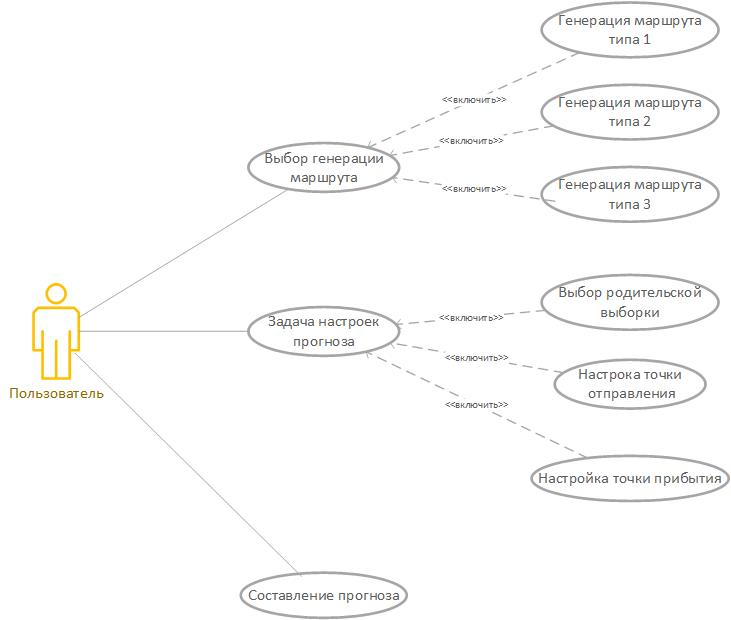
\includegraphics[width  = \linewidth]{gradulation_use-case.jpg}
		\caption{Диаграмма прецедентов}\label{use-case}
	\end{figure}

\appendixtz{Диаграмма последовательности}
	\begin{figure}
		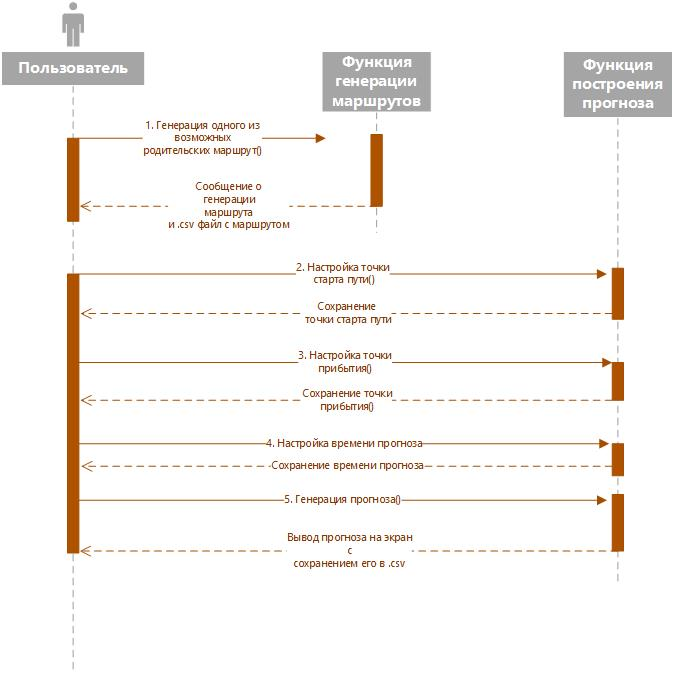
\includegraphics[width  = \linewidth]{gradulation_sequence_pic.jpg}
		\caption{Диаграмма последовательности}\label{sequence}
	\end{figure}
	
\appendixtz{Диаграмма активности}
	\begin{figure}
		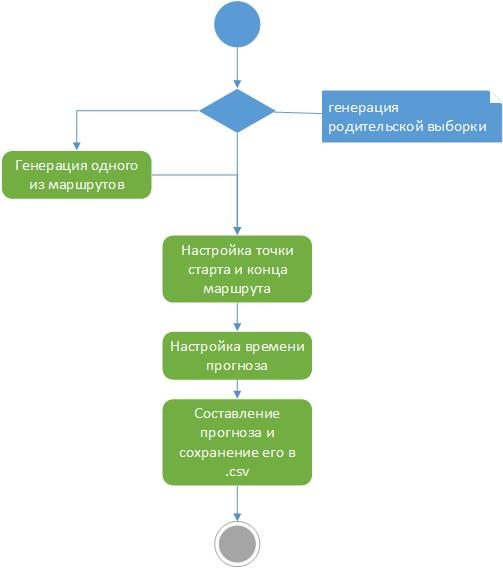
\includegraphics[width  = \linewidth]{gradulation_activity_second.jpg}
		\caption{Диаграмма последовательности}\label{sequence}
	\end{figure}
	
\appendixtz{Диаграмма классов}
	\begin{figure}
		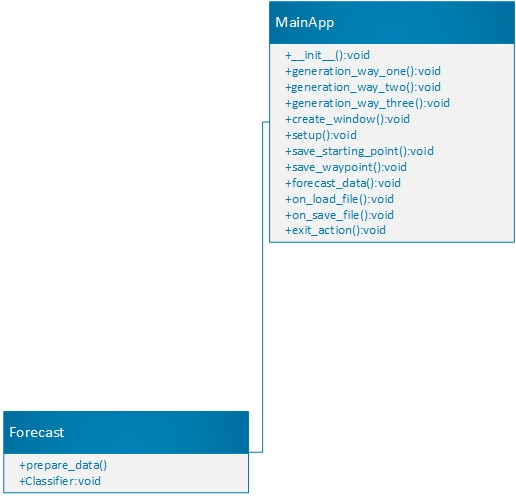
\includegraphics[width  = \linewidth]{gradulation_class_pic.jpg}
		\caption{Диаграмма классов}\label{class}
	\end{figure}
	
\appendixtz{Макет экранных форм}
	\begin{figure}
		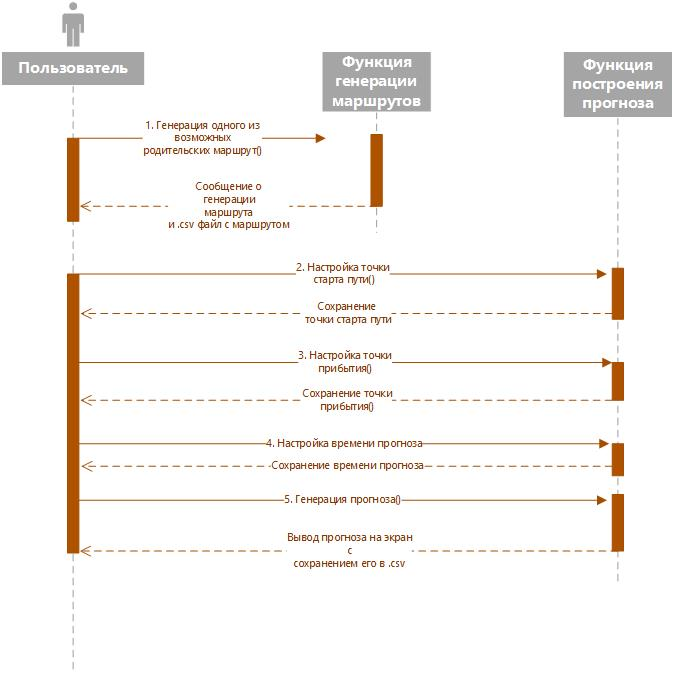
\includegraphics[width  = \linewidth]{gradulation_sequence_pic.jpg}
		\caption{Главное окно}\label{main_window}
	\end{figure}
	
\appendixtz{Тестовый пример для графического интерфейса}
	\par Ход теста:
		\begin{enumerate}
			\item Для того, чтобы создать родительскую выборку:
				\begin{enumerate}
					\item открыть меню приложения
					\item нажать %кнопка меню
					\item выбрать один из пунктов генерации
				\end{enumerate}
			\item Для того, чтобы построить прогноз:
				\begin{enumerate}
					\item заполните поля в в меню  « тут название меню, которое я не помню»
					\item нажмите кнопку «save point»
					\item заполните поля в меню « waypoint»
					\item нажмите кнопку «save waypoint»
					\item введите время прогноза в поле « ещё одно поле, которое я не помню»
					\item нажмите кнопку «forecast»
				\end{enumerate}
			\item сохранить результат в .csv файл и закрыть приложение
		\end{enumerate}
		
\appendixtz{Описание разработанных функций}
	\par В таблице ~\ref{function} расписаны реализованные функции:
	\begin{longtable}{|c|c|}
		\caption {Описание реализованных функций} \label{function} \\ \hline
		    Функция 				&	 Описание 		        \\ \hline \endhead
		   Генерация  родительского	&Генерация маршрута на 60000  записей 	         \\ 
		   маршрута первого типа	& г.Волгоград ул.Грушевская 5 - ВолгГТУ \\ \hline
		   Генерация  родительского	&Генерация маршрута на 60000  записей 	         \\ 
		   маршрута второго типа	& г.Волгоград ул.Грушевская 5 - \\
		   					& г.Волгоград ул.Мясникова 16 \\ \hline
		   Генерация  родительского	&Генерация маршрута на 60000  записей 	         \\ 
		   маршрута третьего типа	& г.Волгоград ул.Грушевская 5 - ВолГУ \\ \hline
		   Функция простроения		&Функция, реализующая прогноз перемещения \\
		   прогноза		 		&в промежутке пути человека \\
		   					&из старта в окончание маршрута \\ 	\hline
		   Функция сохранения 		&Сохранение итогов прогноза         \\	
		   данных в файл	 		&в .csv файл.      	         \\ 	\hline
	\end{longtable}
\end{document}
